\appendix

\renewcommand{\theequation}{\Alph{chapter}-\arabic{equation}}
\renewcommand{\thefigure}{\Alph{chapter}-\arabic{figure}}

\chapter{流体与定温热源的传热计算公式}
\label{cha:CTHX}

假定$U$,$T_{c}$,$\dot{m}$和$c_{p}$都为常数,对于给定的来流温度$T_{i}$,

\begin{figure}[h]
\begin{centering}
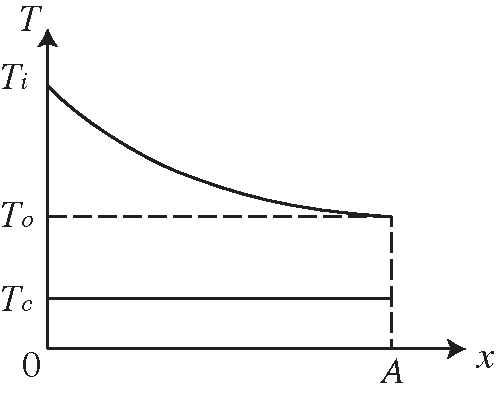
\includegraphics[width=0.4\textwidth]{fig/ConstTempHX.pdf}
\par\end{centering}
\caption{流体与定温热源的传热示意图}
\label{fig:CTHX}
\end{figure}

取$x$为已经参与换热的面积,当$x=0$时,$T(x)=T_i$;当$x=A$时,$T(x)=T_o$。
\begin{equation}
\dot{m}c_{p}dT(x)=(T_{c}-T(x))Udx
\end{equation}

于是,

\begin{equation}
\frac{dT(x)}{dx}=-\frac{U}{\dot{m}c_{p}}(T(x)-T_{c})
\end{equation}

\begin{equation}
T_{g}(x)=T_{p}(x)+T_{h}(x)
\end{equation}
其中,$T_{g}(x)$是通解,$T_{p}(x)$是特解,$T_{h}(x)$是齐次解。

\begin{equation}
-\frac{U}{\dot{m}c_{p}}(T_{p}(x)-T_{c})=0
\end{equation}

\begin{equation}
T_{p}(x)=T_{c}
\end{equation}

\begin{equation}
\frac{dT_{h}(x)}{dx}=-\frac{U}{\dot{m}c_{p}}T_{h}(x)\label{eq:T_h(x)}
\end{equation}

\begin{equation}
\int_{T_{h}(x)=T_{h}(0)}^{T_{h}(x)=T_{h}(A)}\frac{dT_{h}(x)}{T_{h}(x)}=-\int_{x=0}^{x=A}\frac{U}{\dot{m}c_{p}}dx
\end{equation}
\begin{equation}
\frac{T_{h}(A)}{T_{h}(0)}=\exp(-\frac{UA}{\dot{m}c_{p}})
\end{equation}

也就是

\begin{equation}
\frac{T_{g}(A)-T_{p}(A)}{T_{g}(0)-T_{p}(0)}=\exp(-\frac{UA}{\dot{m}c_{p}})
\end{equation}

\begin{equation}
\frac{T_{o}-T_{c}}{T_{i}-T_{c}}=\exp(-\frac{UA}{\dot{m}c_{p}})
\label{eq:Eq}
\end{equation}

\chapter{等热流密度下的流体与定温热源的传热计算公式}
\label{cha:CTCHFHX}

假定$U$,$T_{c}$,$\dot{m}$,$c_p$和$q''$都为常数,对于给定的来流温度${T_i}$,

\begin{figure}[h]
\begin{centering}
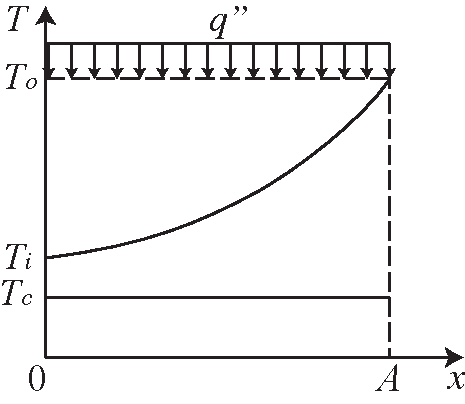
\includegraphics[width=0.4\textwidth]{fig/CTCHFHX.pdf}\caption{等热流密度下的流体与定温热源的传热示意图}
\label{fig:CTCHFHX}
\end{centering}
\end{figure}

取$x$为已经参与换热的面积,当$x=0$时,$T(x)=T_i$;当$x=A$时,$T(x)=T_o$。
\begin{equation}
\dot{m}c_{p}dT(x)=(T_{c}-T(x))Udx+q''dx
\end{equation}

于是,

\begin{equation}
\frac{dT(x)}{dx}=-\frac{UP}{\dot{m}c_{p}}T(x)+\frac{q''P+UPT_{c}}{\dot{m}c_{p}}
\end{equation}
\begin{equation}
T_{g}(x)=T_{p}(x)+T_{h}(x)
\end{equation}
其中,$T_{g}(x)$是通解,$T_{p}(x)$是特解,$T_{h}(x)$是齐次解。

\begin{equation}
-\frac{U}{\dot{m}c_{p}}T_{p}(x)+\frac{q''+UT_{c}}{\dot{m}c_{p}}=0
\end{equation}
\begin{equation}
T_{p}(x)=T_{c}+\frac{q''}{U}
\end{equation}
\begin{equation}
\frac{dT_{h}(x)}{dx}=-\frac{U}{\dot{m}c_{p}}T_{h}(x)
\end{equation}

同\autoref{eq:T_h(x)}一样,于是有
\begin{equation}
\frac{T_{g}(A)-T_{p}(A)}{T_{g}(0)-T_{p}(0)}=\exp(-\frac{UA}{\dot{m}c_{p}})
\end{equation}
\begin{equation}
\frac{T_{o}-T_{c}-\dfrac{q''}{U}}{T_{i}-T_{c}-\dfrac{q''}{U}}=\exp(-\frac{UA}{\dot{m}c_{p}})
\end{equation}

\chapter{类Stream的MATLAB源代码}
\label{cha:MATLAB_SOURCECODE}

%\begin{lstlisting}[language= MATLAB, backgroundcolor = \color{yellow!20}, title = {The MATLAB source code of the definition of the class -- Stream}, label = {lst:MATLAB_SOURCECODE}]
\begin{lstlisting}[language= MATLAB, backgroundcolor = \color{yellow!20}, label = {lst:MATLAB_SOURCECODE}]
classdef Stream < handle
    %Stream This class describes a fluid stream that has inherent
    %properties and dependent properties
    
    properties
        fluid;  % Fluid type
        dot_m;  % Mass flow rate, kg/s
        T;      % Temperature, K
        p;      % Pressure, Pa
        x;      % Quality, [0, 1] for two phase stream; NaN for single 
                %   phase stream
    end
    properties(Dependent)
        h;      % Mass specific enthalpy, J.kg
        s;      % Mass specific entropy, J/kg-K
        cp;     % Specific heat under constant pressure, J/kg-K
    end
    
    methods
        function obj = Stream
            obj.T = Temperature;
            obj.dot_m = Massflow;
            obj.p = Pressure;
        end
        function flowTo(obj, st)
            st.fluid = obj.fluid;
            st.dot_m = obj.dot_m;
        end
        function st2 = mix(obj, st1)
            % Get the properties of a stream mixed by two streams
            % The two streams must have the same fluid type and pressure
            if obj.fluid == st1.fluid
                if  obj.p.v == st1.p.v
                    obj.p = st1.p;
                    st2.fluid = obj.fluid;
                    st2.p = obj.p;
                    st2.dot_m.v = obj.dot_m.v + st1.dot_m.v;
                    h = (obj.dot_m.v .* obj.h + st1.dot_m.v .* st1.h)...
                        ./ (obj.dot_m.v + st1.dot_m.v);
                    st2.T.v = CoolProp.PropsSI('T', 'H', h, 'P',st2.p.v);
                else
                    error('The two streams have different pressures!');
                end
            else
                error('The two streams have different fluid types!');
            end
        end
        function convergeTo(obj, st, y)
            % Get another stream converged (or diverged)
            % from the original stream state.
            % If y < 1, the original stream is diverged
            % If y > 1, the original stream is converged
            st.fluid = obj.fluid;
            st.T = obj.T;
            st.p = obj.p;
            st.x = obj.x;
            st.dot_m.v = obj.dot_m.v .* y;
        end
    end
    methods
        % The dependent properties can be obtained from the inherent
        %   properties
        % If x is NaN, then the dependent properties are determined
        %   by T and P; otherwise, they are determined by P and x
        function value = get.h(obj)
            if isempty(obj.x)
                value = CoolProp.PropsSI('H', 'T', obj.T.v, ...
                    'P', obj.p.v, obj.fluid);
            else
                value = CoolProp.PropsSI('H', 'P', obj.p.v, 'Q', ...
                    obj.x, obj.fluid);
            end
        end
        function value = get.s(obj)
            if isempty(obj.x)
                value = CoolProp.PropsSI('S', 'T', obj.T.v, ...
                    'P', obj.p.v, obj.fluid);
            else
                value = CoolProp.PropsSI('S', 'P', obj.p.v, 'Q', ...
                    obj.x, obj.fluid);
            end
        end
        function value = get.cp(obj)
            if isempty(obj.x)
                value = CoolProp.PropsSI('C', 'T', obj.T.v, ...
                    'P', obj.p.v, obj.fluid);
            else
                value = inf;
            end
        end
    end
end
\end{lstlisting}
  
\begin{publications}
	\begin{spacing}{1.4}
  \item Cheng Zhang, Yanping Zhang, Inmaculada Arauzo, et al. Cascade system using both trough system and dish system for power generation. Energy Conversion and Management, 2017. 142:494–503
  \item Cheng Zhang, Yanping Zhang, Xiaolin Lei, et al. Design and Comparison of Solar Thermal Oilfield Steam Production System Plans. Journal of Solar Energy Engineering, 2017. 139:1-4
  \item Cheng Zhang, Kun Wang, Jizhou Wang, et al. FEA simulation on the alignment of the shafts of three-fulcrum turbine. International Conference on Power Engineering. 2013. Wuhan.
  \item Chongzhe Zou, Yanping Zhang, Quentin Falcoz, et al. Design and Optimization of a High-temperature Cavity Receiver for a Solar Energy Cascade Utilization System. Renewable Energy, 2017. 103:478-489
  \item Chongzhe Zou, Yanping Zhang, Huayi Feng, et al. Effects of Geometrical Parameters on Thermal Performance for a Cylindrical Solar Receiver Using 3D numerical Model. Energy Conversion and Management, 2017. 149:293-302
  
  \item 张燕平,张成,黄树红. 一种采用换热系统对被加热流体进行分阶段加热的流量控制方法. 中国,发明专利, 201610805604.2,2018
  \item 张燕平,张成,黄树红. 一种太阳能光热联合发电系统. 中国,发明专利,201610806296.5,2018
  \item 张燕平,张成. 太阳能光热发电开发系统. 中国,软件著作权,2017SR382378,2017		
	\end{spacing}
\end{publications}